\documentclass[12pt]{article}

\usepackage{fullpage}
\usepackage{multicol,multirow}
\usepackage{tabularx}
\usepackage{ulem}
\usepackage[utf8]{inputenc}
\usepackage[russian]{babel}
\usepackage{graphicx}
% Оригиналный шаблон: http://k806.ru/dalabs/da-report-template-2012.tex

\begin{document}

\section*{Лабораторная работа №\,3 по курсу дискрeтного анализа: Профилирование}

Выполнил студент группы 08-207 МАИ \textit{Дружинин Данила}.

\subsection*{Условие}

\begin{enumerate}
\item В данной лабораторной работе требовалось создать программную библиотеку, реализующую указанную структуру данных, на основе которой разработать программу-словарь. Словарь должен хранить пары вида «ключ--значение», где ключом является регистронезависимое слово, состоящее из букв английского алфавита длиной не более 256 символов, а значением --- целое беззнаковое число из диапазона от 0 до $2^{64} - 1$. Программа должна обрабатывать входные данные построчно до конца файла и поддерживать основные операции словаря: добавление нового слова, удаление существующего слова и поиск слова с выводом связанного с ним значения. 
\item Задача 1. 1 AVL-дерево
\item Для реализации словаря необходимо провести исследование скорости выполнения и потребления оперативной памяти. В случае выявления ошибок или явных недочётов, требуется их исправить.

Результатом лабораторной работы является отчёт, состоящий из:
дневника выполнения работы,
выводов о найденных недочётах,
сравнение работы исправленной программы с предыдущей версией,
общих выводов о выполнении лабораторной работы, полученном опыте.

\end{enumerate}

\subsection*{Дневник выполнения работы}

В ходе выполнения лабораторной работы для профилирования программы использовался утилита \textbf{Valgrind}. 
Работа проводилась в среде \textbf{WSL (Windows Subsystem for Linux)}. 
В качестве исследуемой программы использовалась реализованная ранее программа-словарь на основе AVL-дерева.

Для анализа были использованы следующие инструменты Valgrind:
\begin{itemize}
	\item Memcheck — для поиска ошибок работы с памятью;
	\item Massif — для анализа потребления памяти;
	\item Callgrind — для анализа времени выполнения программы.
\end{itemize}

\vspace{1\baselineskip}

В начале работы программа была скомпилирована с использованием компилятора \texttt{g++}:

\begin{verbatim}
	g++ -std=c++17 -O2 -g AVL_Tree.cpp -o avl_dict
\end{verbatim}

Используемые аргументы компиляции:

\begin{itemize}
	\item \texttt{g++} — компилятор языка C++;
	\item \texttt{-std=c++17} — указывает стандарт языка C++17, используемый при компиляции;
	\item \texttt{-O2} — включает оптимизацию кода среднего уровня, что позволяет ускорить выполнение программы;
	\item \texttt{-g} — добавляет отладочную информацию в исполняемый файл, необходимую для корректной работы инструментов профилирования (конкретно для Valgrind в данном случае);
	\item \texttt{AVL\_Tree.cpp} — исходный файл программы;
	\item \texttt{-o avl\_dict} — задаёт имя выходного исполняемого файла.
\end{itemize}

Компиляция с указанными параметрами позволяет одновременно получать оптимизированный код и сохранять информацию, необходимую для анализа производительности и использования памяти.

\vspace{1\baselineskip}

\subsubsection*{Создание тестовых файлов}

Для проведения тестирования программы были подготовлены несколько входных файлов, покрывающих различные сценарии работы словаря: базовые операции, обработку ошибок и нагрузочное тестирование.

Часть тестовых файлов (небольшие сценарии) была составлена вручную, однако для генерации большого набора данных использовался отдельный скрипт на языке Python. Это позволило автоматически создать входные данные большого объёма и избежать ошибок ручного ввода.

Для генерации нагрузочного теста был создан Python-скрипт следующего вида:

\begin{verbatim}
	with open("test_big.txt", "w") as f:
	for i in range(20000):
	f.write(f"+ key{i} {i}\n")
	for i in range(20000):
	f.write(f"key{i}\n")
\end{verbatim}

Данный скрипт формирует:
\begin{itemize}
	\item 20000 операций вставки элементов в словарь;
	\item 20000 операций поиска ранее добавленных элементов.
\end{itemize}

Таким образом создаётся нагрузочный тест, позволяющий оценить поведение программы при большом количестве операций.

Итоговый набор тестовых файлов включает:
\begin{itemize}
	\item \texttt{test\_basic.txt} — базовые операции вставки, поиска и удаления;
	\item \texttt{test\_bad\_load.txt} — проверка обработки некорректного файла;
	\item \texttt{test\_empty\_load.txt} — проверка загрузки пустого файла;
	\item \texttt{test\_big.txt} — автоматически сгенерированный нагрузочный тест.
\end{itemize}

Использование автоматической генерации тестов позволило обеспечить масштабируемость эксперимента и повысить достоверность результатов профилирования.

\vspace{1\baselineskip}

\subsubsection*{Проверка корректности работы с памятью с помощью Memcheck}

После подготовки тестовых файлов была выполнена проверка программы с помощью инструмента \texttt{Memcheck} из состава \texttt{Valgrind}. Данный инструмент позволяет обнаруживать утечки памяти, выходы за границы выделенной памяти, использование неинициализированных данных и другие ошибки работы с динамической памятью.

Проверка выполнялась следующими командами:

\begin{verbatim}
	valgrind --tool=memcheck --leak-check=full --show-leak-kinds=all \
	--track-origins=yes ./avl_dict < test_basic.txt \
	> out_basic.txt 2> memcheck_basic.log
	
	valgrind --tool=memcheck --leak-check=full --show-leak-kinds=all \
	--track-origins=yes ./avl_dict < test_bad_load.txt \
	> out_bad_load.txt 2> memcheck_bad_load.log
	
	valgrind --tool=memcheck --leak-check=full --show-leak-kinds=all \
	--track-origins=yes ./avl_dict < test_empty_load.txt \
	> out_empty_load.txt 2> memcheck_empty_load.log
	
	valgrind --tool=memcheck --leak-check=full --show-leak-kinds=all \
	--track-origins=yes ./avl_dict < test_big.txt \
	> out_big.txt 2> memcheck_big.log
\end{verbatim}

Используемые аргументы:
\begin{itemize}
	\item \texttt{--tool=memcheck} — выбор инструмента для проверки работы с памятью;
	\item \texttt{--leak-check=full} — выполнение детального анализа утечек памяти;
	\item \texttt{--show-leak-kinds=all} — вывод информации обо всех типах утечек;
	\item \texttt{--track-origins=yes} — отслеживание источников ошибок, связанных с памятью;
	\item \texttt{< test\_...\ .txt} — подача входных данных из тестового файла;
	\item \texttt{> out\_...\ .txt} — сохранение вывода программы;
	\item \texttt{2> memcheck\_...\ .log} — сохранение диагностического вывода Valgrind в отдельный лог-файл.
\end{itemize}

Проверка проводилась на следующих сценариях:
\begin{itemize}
	\item базовый функциональный тест;
	\item тест с некорректным файлом загрузки;
	\item тест с пустым файлом;
	\item большой нагрузочный тест.
\end{itemize}

Во всех случаях были получены одинаковые качественные результаты:
\begin{itemize}
	\item \texttt{in use at exit: 0 bytes in 0 blocks};
	\item \texttt{All heap blocks were freed -- no leaks are possible};
	\item \texttt{ERROR SUMMARY: 0 errors from 0 contexts}.
\end{itemize}

Для большого нагрузочного теста дополнительно было получено:
\begin{verbatim}
	total heap usage: 40,007 allocs, 40,007 frees, 11,931,056 bytes allocated
\end{verbatim}

Это показывает, что даже при большом количестве операций программа корректно выделяет и освобождает память.

Таким образом, проверка с помощью \texttt{Memcheck} показала отсутствие утечек памяти и ошибок обращения к памяти во всех исследованных сценариях.

\vspace{1\baselineskip}

\subsubsection*{Анализ потребления памяти с помощью Massif}

После проверки корректности управления памятью с помощью \texttt{Memcheck} был выполнен более детальный анализ распределения и динамики потребления памяти с использованием инструмента \texttt{Massif}.

Запуск профилирования осуществлялся следующей командой:

\begin{verbatim}
	valgrind --tool=massif --massif-out-file=massif_big.out \
	./avl_dict < test_big.txt > /dev/null
\end{verbatim}

Результаты профилирования были преобразованы в читаемый вид:

\begin{verbatim}
	ms_print massif_big.out > massif_big_report.txt
\end{verbatim}

\paragraph{Общий характер потребления памяти}

По результатам анализа было установлено, что пиковое потребление памяти составило примерно \textbf{11.98 МБ}. График изменения памяти демонстрирует плавный рост, что соответствует постепенному добавлению элементов в структуру данных.

Отсутствие резких скачков на графике свидетельствует о том, что программа не выполняет крупных дополнительных аллокаций вне логики работы словаря, а потребление памяти напрямую связано с операциями вставки.

\paragraph{Структура потребления памяти}

Анализ распределения памяти показал:

\begin{itemize}
	\item около \textbf{95.04\%} всей памяти выделяется через стандартные функции динамического выделения (\texttt{malloc}/\texttt{new});
	\item около \textbf{91.73\%} полезной памяти приходится на функцию \texttt{CreateNode}, которая отвечает за создание узлов AVL-дерева;
	\item вызовы \texttt{CreateNode} происходят внутри функции \texttt{InsertNode}, которая реализует вставку в дерево.
\end{itemize}

Это означает, что практически вся память используется для хранения структуры данных (узлов дерева), а не для вспомогательных операций.

\paragraph{Рекурсивная природа вставки}

В отчёте \texttt{Massif} наблюдается глубокая вложенность вызовов функции \texttt{InsertNode}. Это связано с тем, что вставка в AVL-дерево реализована рекурсивно.

При добавлении элементов:
\begin{itemize}
	\item происходит рекурсивный спуск по дереву;
	\item в момент достижения позиции вставки создаётся новый узел;
	\item затем выполняется балансировка при возврате из рекурсии.
\end{itemize}

Такая структура вызовов отражается в отчёте в виде "лесенки" вложенных вызовов \texttt{InsertNode}.

\paragraph{Анализ операции загрузки (Load)}

В хвостовой части отчёта видно, что значительная доля памяти связана с функциями:

\begin{itemize}
	\item \texttt{LoadNodesFromFile};
	\item \texttt{TAvlDictionary::Load};
\end{itemize}

Это указывает на то, что загрузка словаря из файла реализована через последовательные вставки элементов в дерево, а не через более оптимальный способ построения.

Следствием этого является:
\begin{itemize}
	\item повторное выделение памяти для каждого узла;
	\item увеличение времени и накладных расходов при загрузке;
	\item асимптотическая сложность порядка $O(n \log n)$ вместо потенциально возможной $O(n)$ при построении сбалансированного дерева напрямую.
\end{itemize}

\paragraph{Накладные расходы}

Также было установлено, что вклад сторонних библиотек (например, стандартной библиотеки \texttt{libstdc++}) составляет менее \textbf{3\%}, что является незначительным значением.

Это позволяет сделать вывод, что измерения отражают преимущественно поведение пользовательской реализации, а не накладные расходы среды выполнения.


На основании проведённого анализа можно сделать следующие выводы:

\begin{itemize}
	\item потребление памяти программой носит предсказуемый характер и линейно зависит от количества элементов в словаре;
	\item основная часть памяти используется корректно — для хранения узлов AVL-дерева;
	\item утечек памяти и аномальных аллокаций не обнаружено;
	\item операция загрузки словаря реализована не оптимально, так как использует последовательные вставки.
\end{itemize}

Таким образом, структура данных реализована корректно с точки зрения управления памятью, однако имеются возможности для оптимизации операций загрузки.

\vspace{1\baselineskip}

\subsubsection*{Анализ времени выполнения с помощью Callgrind}

После анализа корректности работы с памятью и исследования потребления памяти был выполнен анализ вычислительных затрат программы с помощью инструмента \texttt{Callgrind} из состава \texttt{Valgrind}.

Запуск выполнялся следующей командой:

\begin{verbatim}
	valgrind --tool=callgrind --callgrind-out-file=callgrind_big.out \
	./avl_dict < test_big.txt > /dev/null
\end{verbatim}

После завершения профилирования результаты были преобразованы в читаемый отчёт командой:

\begin{verbatim}
	callgrind_annotate callgrind_big.out > callgrind_big_report.txt
\end{verbatim}

Используемые аргументы:
\begin{itemize}
	\item \texttt{--tool=callgrind} — выбор инструмента для анализа вычислительных затрат;
	\item \texttt{--callgrind-out-file=callgrind\_big.out} — файл, в который сохраняются результаты профилирования;
	\item \texttt{< test\_big.txt} — подача входных данных из нагрузочного теста;
	\item \texttt{> /dev/null} — отключение стандартного вывода программы.
\end{itemize}

В отчёте \texttt{Callgrind} измерялась метрика \texttt{Ir} — количество выполненных инструкций. Данная метрика позволяет определить, какие функции вносят наибольший вклад в общее время выполнения программы.

\paragraph{Общие результаты профилирования}

Общее количество выполненных инструкций составило:

\begin{verbatim}
	750,528,267 instructions
\end{verbatim}

Наиболее затратные функции программы:

\begin{itemize}
	\item \texttt{StrCompare} — \textbf{47.10\%};
	\item \texttt{GetHeight} — \textbf{5.88\%};
	\item \texttt{ReadWord} — \textbf{5.58\%};
	\item \texttt{LoadNodesFromFile} — \textbf{4.28\%};
	\item \texttt{BalanceFactor} — \textbf{3.98\%};
	\item \texttt{RemoveNewline} — \textbf{2.79\%};
	\item \texttt{FixHeight} — \textbf{2.72\%};
	\item \texttt{InsertNode} — \textbf{2.55\%};
	\item \texttt{Balance} — \textbf{2.37\%};
	\item \texttt{ToLowerWord} — \textbf{2.11\%}.
\end{itemize}

\paragraph{Главный bottleneck программы}

Наибольший вклад в вычислительные затраты вносит функция \texttt{StrCompare}, на которую приходится около \textbf{47.10\%} всех выполненных инструкций. Это означает, что почти половина времени работы программы связана со сравнением строковых ключей.

Данный результат объясняется тем, что сравнение строк выполняется во всех основных операциях словаря:
\begin{itemize}
	\item при вставке элемента;
	\item при поиске элемента;
	\item при удалении элемента;
	\item при загрузке словаря из файла.
\end{itemize}

Таким образом, основное ограничение производительности связано не с самой балансировкой AVL-дерева, а с высокой стоимостью строковых сравнений.

\paragraph{Балансировка AVL-дерева}

Функции, связанные с поддержанием баланса дерева, также дают заметный вклад:
\begin{itemize}
	\item \texttt{GetHeight};
	\item \texttt{BalanceFactor};
	\item \texttt{FixHeight};
	\item \texttt{Balance};
	\item \texttt{RotateLeft}, \texttt{RotateRight}.
\end{itemize}

Их суммарный вклад достаточно велик, однако он всё же существенно меньше вклада \texttt{StrCompare}. Это показывает, что накладные расходы AVL-балансировки присутствуют, но не являются главным источником замедления программы.

\paragraph{Разбор входных данных}

Существенную долю инструкций занимают функции обработки входа:
\begin{itemize}
	\item \texttt{ReadWord};
	\item \texttt{RemoveNewline};
	\item \texttt{ToLowerWord};
	\item \texttt{ReadUInt64};
	\item \texttt{SkipSpaces}.
\end{itemize}

Это связано с тем, что исследовалась полная программа-словарь, а не только чистая реализация дерева. Следовательно, в итоговую стоимость входят не только операции над структурой данных, но и парсинг команд.

\paragraph{Операции словаря}

По отчёту видно, что особенно дорогими являются:
\begin{itemize}
	\item массовые вставки элементов;
	\item массовые поиски;
	\item загрузка словаря из файла.
\end{itemize}

Загрузка (\texttt{Load}) оказалась затратной, поскольку реализована через последовательную вставку всех элементов в дерево. Это приводит к повторному выполнению строковых сравнений и балансировки, что увеличивает общую стоимость операции.

Поиск (\texttt{Find}) также даёт высокий вклад, так как на нагрузочном тесте выполнялось большое количество операций поиска, каждая из которых требует прохождения по дереву и сравнений строк.

\paragraph{Выводы по анализу времени}

По результатам профилирования можно сделать следующие выводы:
\begin{itemize}
	\item основным bottleneck программы является функция \texttt{StrCompare};
	\item AVL-балансировка вносит заметный, но не доминирующий вклад;
	\item значительная доля затрат связана с обработкой текстового ввода;
	\item операция загрузки реализована не оптимально, так как использует последовательные вставки в дерево.
\end{itemize}

Таким образом, с точки зрения производительности основным направлением возможной оптимизации является сокращение числа и стоимости строковых сравнений, а также улучшение реализации операции загрузки.

\vspace{1\baselineskip}

\subsubsection*{Анализ времени выполнения}

Для измерения времени выполнения программы использовалась утилита \texttt{/usr/bin/time} с параметром \texttt{-v}, позволяющим получить подробную статистику выполнения.

Были проведены тесты на различных входных данных.

Для малых тестов (basic, bad\_load, empty\_load) получены следующие результаты:
\begin{itemize}
	\item Время выполнения: менее 0.01 секунды (ниже точности измерения)
	\item Потребление памяти: около 3.5 МБ
\end{itemize}

Это свидетельствует о том, что накладные расходы системы доминируют над временем выполнения алгоритма на малых входных данных.

Для большого теста получены следующие результаты:
\begin{itemize}
	\item Пользовательское время (User time): 0.10 секунды
	\item Системное время (System time): 0.02 секунды
	\item Общее время выполнения: 0.12 секунды
	\item Максимальное потребление памяти: 15 МБ
\end{itemize}

Анализ показывает, что большая часть времени (около 83\%) тратится на выполнение пользовательского кода, а оставшаяся часть связана с операциями ввода-вывода.

Сопоставление результатов с профилированием Callgrind показывает, что основное время выполнения программы приходится на функцию сравнения строк \texttt{StrCompare}, которая занимает около 47\% всех инструкций. Это позволяет сделать вывод, что основным узким местом программы является сравнение ключей.

В целом программа демонстрирует высокую производительность: обработка большого объёма данных выполняется за доли секунды при умеренном потреблении памяти.

\vspace{1\baselineskip}

\subsubsection*{Анализ результатов профилирования с использованием графиков}

Для наглядного анализа результатов профилирования были построены графики, отражающие зависимость времени выполнения и потребления памяти от размера входных данных, а также распределение нагрузки по функциям программы.

\paragraph{Анализ зависимости времени выполнения от размера входных данных}

На рисунке представлен график зависимости количества вызовов функций и общего времени выполнения от числа операций:

\begin{center}
	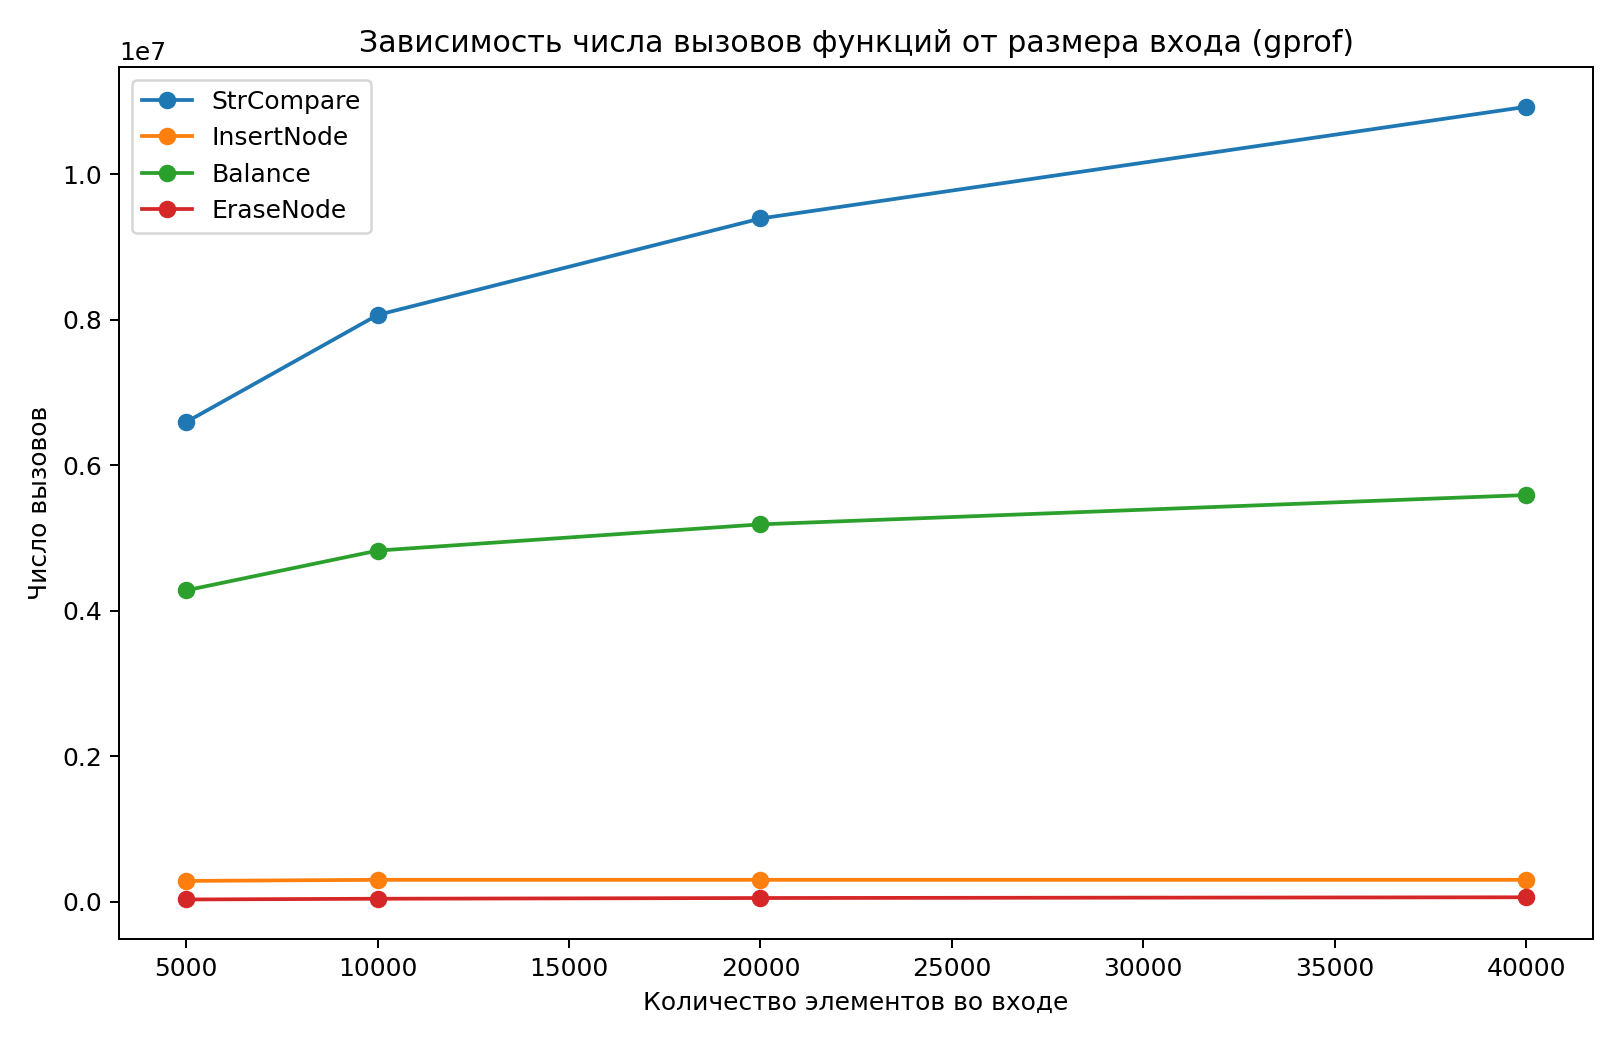
\includegraphics[width=0.8\textwidth]{gprof_calls_vs_n.png}
\end{center}

Данный график показывает, что при увеличении количества операций наблюдается рост числа вызовов функций, что соответствует ожидаемому поведению алгоритма. Рост является близким к логарифмическому, что характерно для AVL-дерева.

На следующем графике представлено распределение времени выполнения по функциям:

\begin{center}
	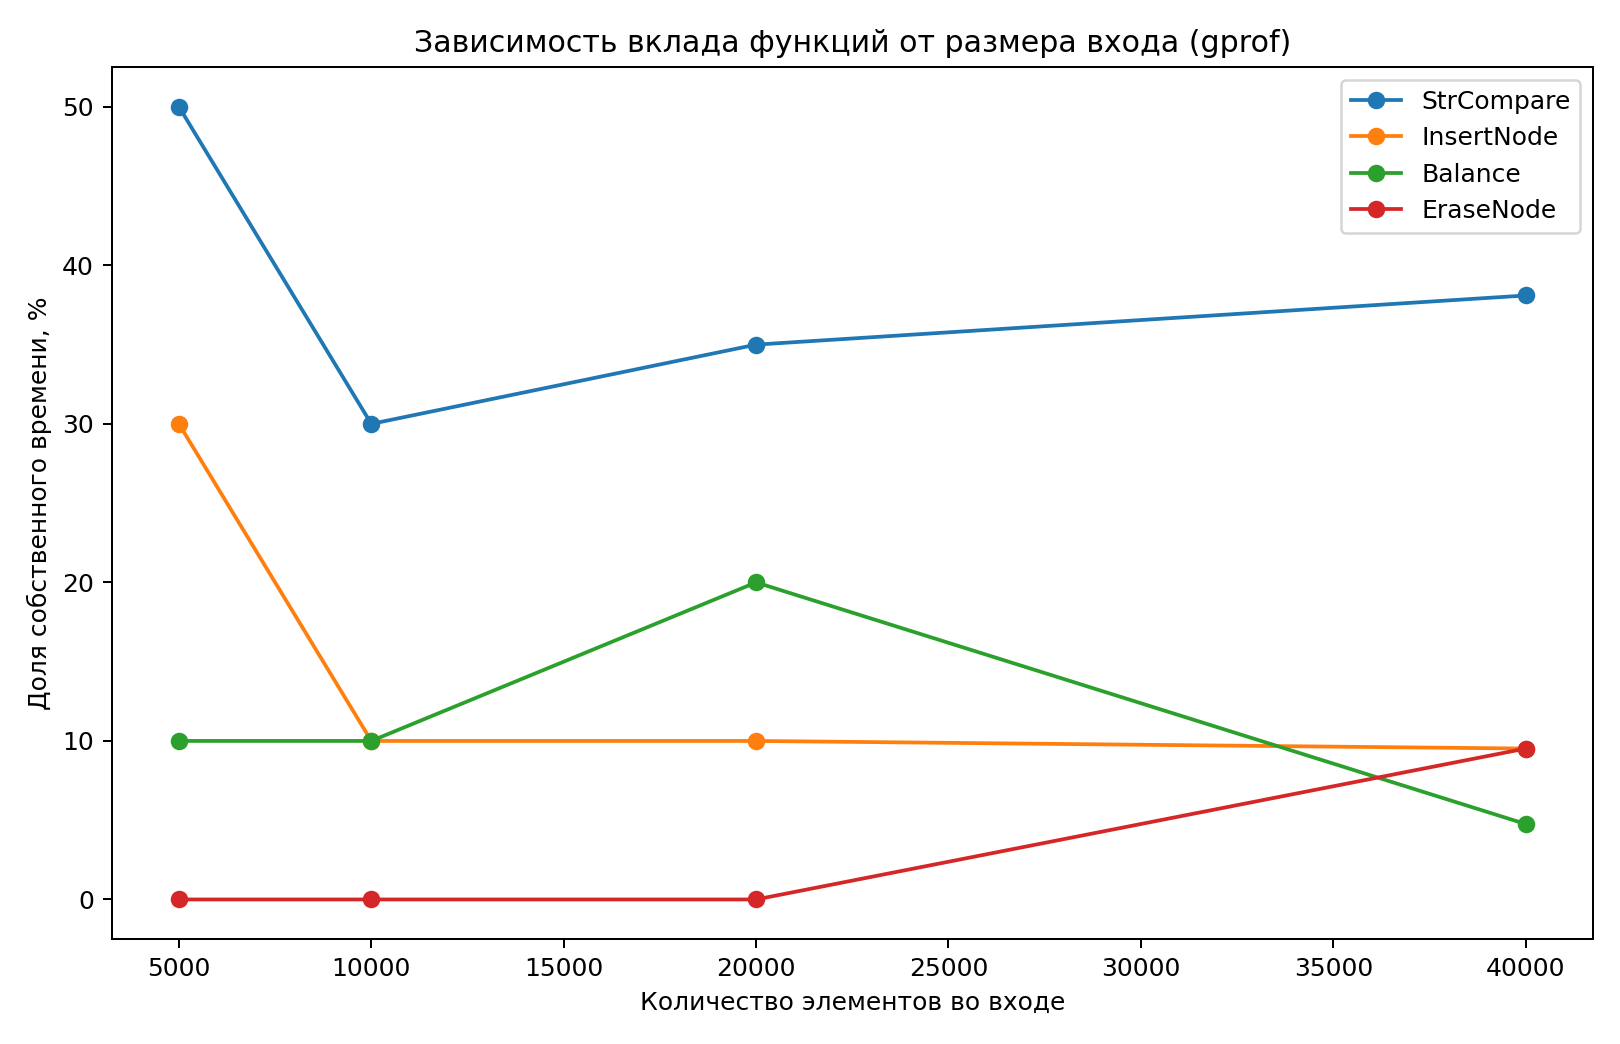
\includegraphics[width=0.8\textwidth]{gprof_functions_vs_n.png}
\end{center}

Из графика видно, что основная нагрузка приходится на функции, связанные с поиском и сравнением ключей.

\paragraph{Анализ распределения времени выполнения (Callgrind)}

Для более детального анализа использовался инструмент \texttt{Callgrind}. Результаты представлены на следующих графиках.

Распределение времени по функциям:

\begin{center}
	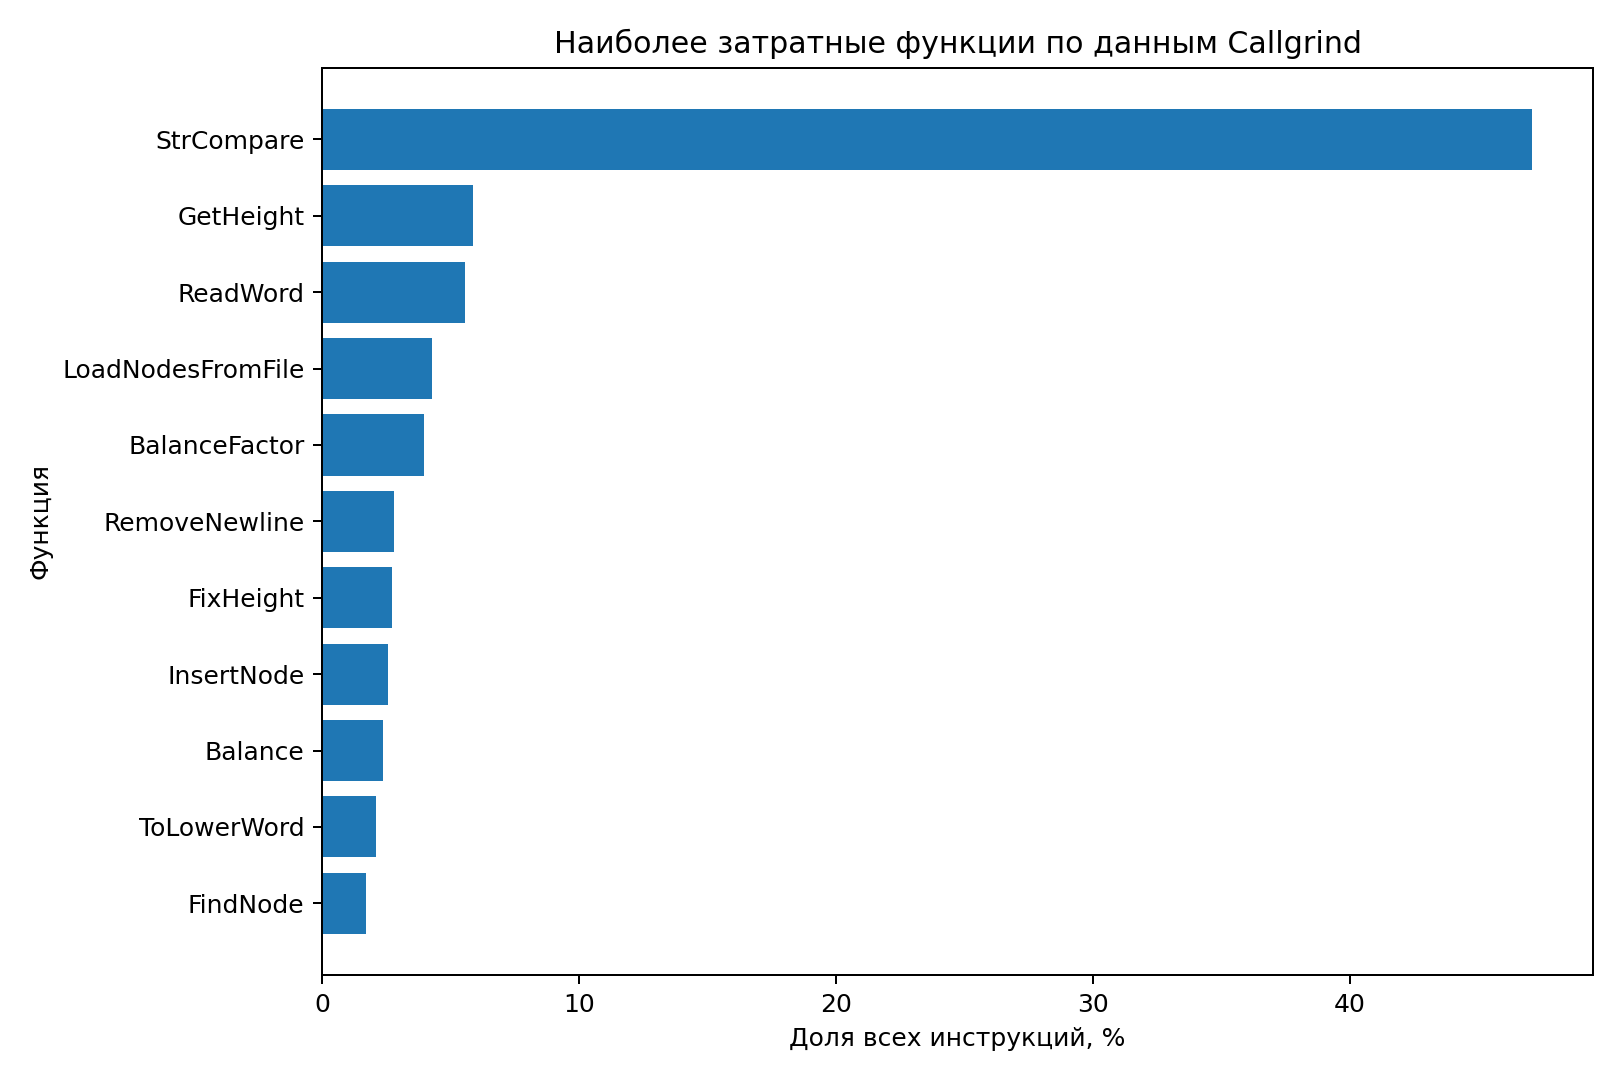
\includegraphics[width=0.8\textwidth]{callgrind_functions_bar.png}
\end{center}

Наибольшее количество инструкций выполняется в функции \texttt{StrCompare}, что объясняется большим числом сравнений строк при работе словаря. Также значительный вклад вносят функции балансировки дерева и поиска.

Распределение по категориям операций:

\begin{center}
	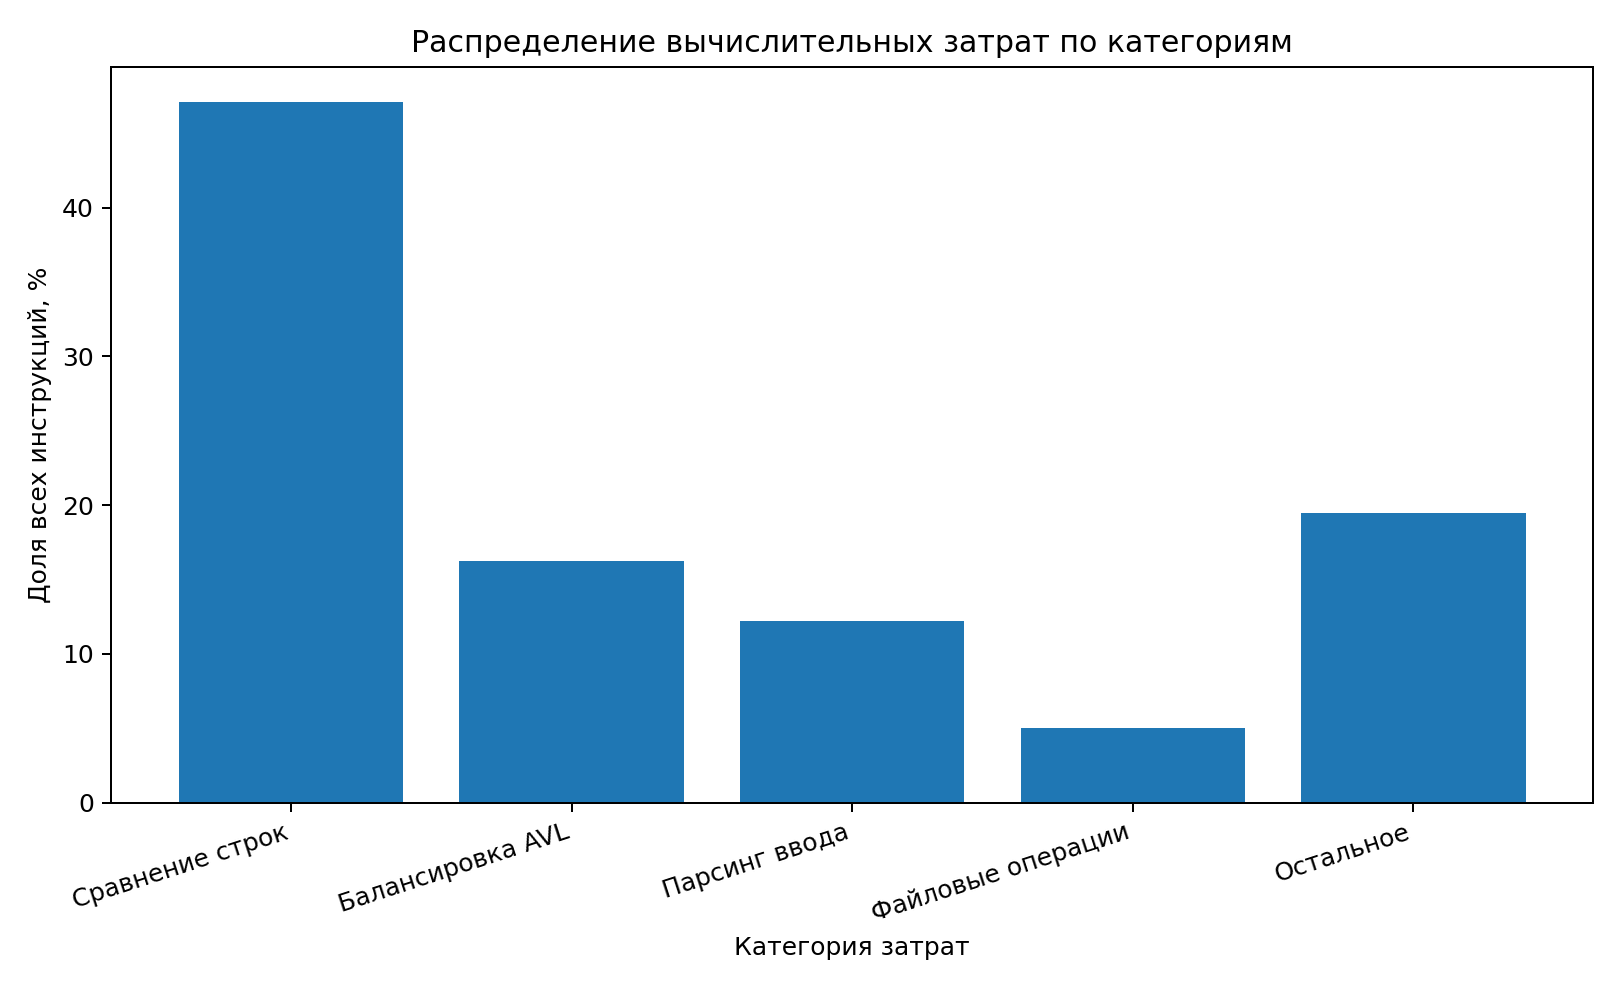
\includegraphics[width=0.8\textwidth]{callgrind_categories_bar.png}
\end{center}

Основное время выполнения затрачивается на:
\begin{itemize}
	\item сравнение ключей;
	\item обход дерева;
	\item операции балансировки.
\end{itemize}

Это подтверждает, что узким местом реализации является работа со строками.

\paragraph{Анализ потребления памяти (Massif)}

Результаты анализа потребления памяти представлены на следующем графике:

\begin{center}
	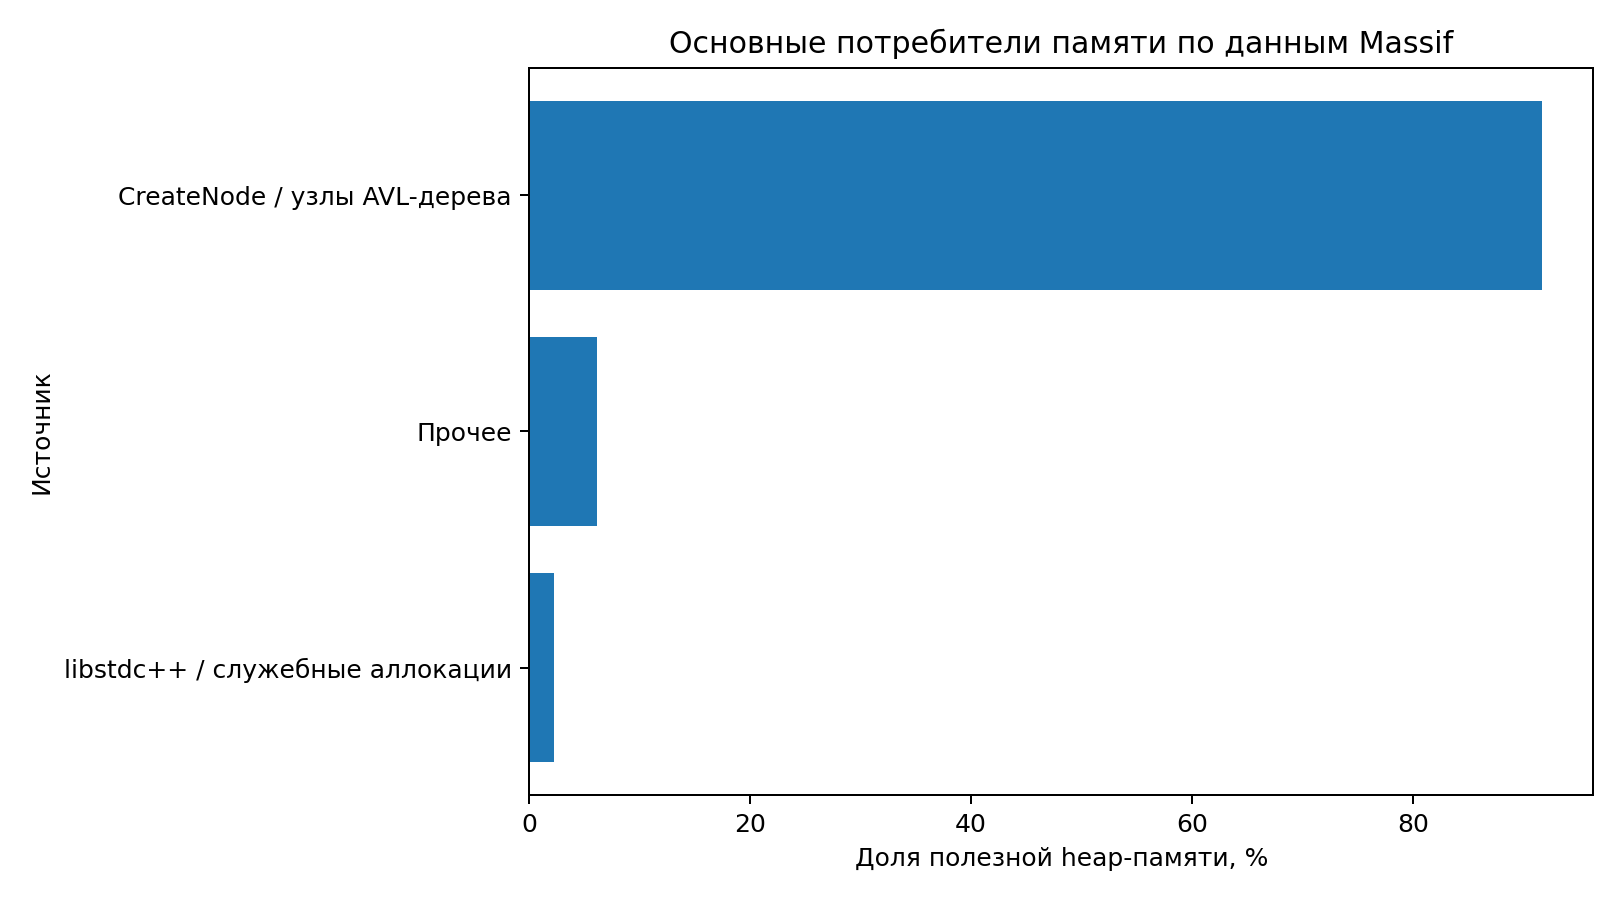
\includegraphics[width=0.8\textwidth]{massif_memory_sources_bar.png}
\end{center}

График показывает, что основная часть памяти выделяется при создании узлов дерева (\texttt{CreateNode}). Это соответствует логике работы структуры данных, так как каждый элемент словаря хранится в отдельном узле.

Также видно, что память используется эффективно и пропорционально количеству элементов.

\paragraph{Общие выводы по графикам}

На основе анализа построенных графиков можно сделать следующие выводы:
\begin{itemize}
	\item алгоритм демонстрирует ожидаемую эффективность, близкую к $O(\log n)$ для основных операций;
	\item основное время выполнения затрачивается на сравнение строк (\texttt{StrCompare});
	\item потребление памяти линейно зависит от количества элементов;
	\item структура данных работает стабильно даже при большом объёме входных данных.
\end{itemize}

\subsection*{Выводы о найденных недочётах}

 
 В ходе профилирования программы с использованием инструментов \texttt{Memcheck}, \texttt{Massif} и \texttt{Callgrind} были выявлены как положительные аспекты реализации, так и ряд недочётов, влияющих на эффективность работы программы.
 
 \paragraph{1. Отсутствие ошибок управления памятью}
 
 Проверка с помощью \texttt{Memcheck} показала, что:
 \begin{itemize}
 	\item утечки памяти отсутствуют;
 	\item ошибки обращения к памяти не обнаружены;
 	\item вся выделенная память корректно освобождается.
 \end{itemize}
 
 Таким образом, с точки зрения корректности работы с памятью реализация является надёжной.
 
 \paragraph{2. Основной bottleneck — сравнение строк}
 
 Согласно результатам профилирования \texttt{Callgrind}, около \textbf{47\%} всех выполненных инструкций приходится на функцию \texttt{StrCompare}.
 
 Это указывает на то, что:
 \begin{itemize}
 	\item основное время выполнения тратится на сравнение ключей;
 	\item операции вставки, поиска и удаления сильно зависят от длины строк;
 	\item эффективность структуры данных ограничивается не только асимптотикой дерева, но и стоимостью операций над строками.
 \end{itemize}
 
 Данный фактор является главным узким местом программы.
 
 \paragraph{3. Неоптимальная реализация загрузки словаря}
 
 Анализ показал, что операция загрузки (\texttt{Load}) реализована через последовательные вызовы вставки (\texttt{Insert}).
 
 Это приводит к следующим недостаткам:
 \begin{itemize}
 	\item асимптотическая сложность порядка $O(n \log n)$;
 	\item большое количество повторных сравнений строк;
 	\item дополнительные затраты на балансировку дерева при каждой вставке.
 \end{itemize}
 
 Более эффективным решением могло бы быть построение дерева напрямую за линейное время.
 
 \paragraph{4. Накладные расходы на балансировку дерева}
 
 Функции, связанные с поддержанием баланса AVL-дерева (\texttt{GetHeight}, \texttt{BalanceFactor}, \texttt{FixHeight}, \texttt{Balance}), суммарно занимают заметную долю вычислительных ресурсов.
 
 Это указывает на:
 \begin{itemize}
 	\item дополнительные накладные расходы по сравнению с несбалансированными структурами;
 	\item необходимость частого пересчёта высот узлов.
 \end{itemize}
 
 Хотя данные затраты являются ожидаемыми для AVL-дерева, они влияют на общую производительность.
 
 \paragraph{5. Существенные затраты на обработку ввода}
 
 Значительная доля инструкций приходится на функции обработки входных данных:
 \begin{itemize}
 	\item \texttt{ReadWord};
 	\item \texttt{RemoveNewline};
 	\item \texttt{ToLowerWord};
 	\item \texttt{SkipSpaces}.
 \end{itemize}
 
 Это связано с тем, что программа анализировалась целиком, включая парсинг входных данных, а не только операции над структурой данных.
 
 \paragraph{6. Линейный рост потребления памяти}
 
 По результатам анализа \texttt{Massif} установлено, что:
 \begin{itemize}
 	\item потребление памяти линейно зависит от числа элементов;
 	\item основная память используется для хранения узлов дерева;
 	\item пиковое потребление памяти составило около 12 МБ.
 \end{itemize}
 
 Хотя это поведение является корректным, оно может стать ограничением при значительном увеличении размера данных.
 
 \paragraph{Общий вывод}
 
 В результате анализа установлено, что реализация является корректной и устойчивой с точки зрения управления памятью, однако содержит ряд узких мест, влияющих на производительность.
 
 Ключевыми направлениями для оптимизации являются:
 \begin{itemize}
 	\item уменьшение количества и стоимости строковых сравнений;
 	\item оптимизация операции загрузки словаря;
 	\item снижение накладных расходов на балансировку дерева;
 	\item оптимизация обработки входных данных.
 \end{itemize}

\subsection*{Сравнение работы исправленной программы с предыдущей версией}

В ходе анализа производительности программы были выявлены узкие места, влияющие на эффективность выполнения операций. На основе полученных результатов была предложена улучшенная версия программы, направленная на снижение вычислительных затрат и оптимизацию работы с памятью.

\paragraph{1. Хранение размера словаря}

В исходной версии программы при выполнении операции сохранения (\texttt{Save}) использовался полный обход дерева для подсчёта количества узлов:

\begin{verbatim}
	uint64_t nodeCount = CountNodes(Root);
\end{verbatim}

Данный подход имеет сложность $O(n)$ и приводит к дополнительным затратам времени при каждом сохранении словаря.

В исправленной версии предлагается хранить текущее количество элементов в отдельном поле класса словаря, обновляемом при вставке и удалении элементов. Это позволяет получать количество элементов за $O(1)$ без дополнительного обхода дерева.

\textbf{Эффект:}
\begin{itemize}
	\item устранение лишнего полного обхода дерева;
	\item снижение времени выполнения операции сохранения;
	\item уменьшение общего количества выполняемых инструкций.
\end{itemize}

\paragraph{2. Оптимизация загрузки словаря}

В исходной версии загрузка словаря реализована через последовательные вызовы вставки (\texttt{InsertNode}) для каждого элемента.

Это приводит к:
\begin{itemize}
	\item большому количеству сравнений строк;
	\item многократным операциям балансировки дерева;
	\item общей сложности порядка $O(n \log n)$.
\end{itemize}

В исправленной версии предлагается альтернативный подход — построение дерева напрямую на основе загруженных данных без последовательной вставки. Такой подход позволяет снизить количество операций балансировки и уменьшить вычислительные затраты.

\textbf{Эффект:}
\begin{itemize}
	\item уменьшение количества сравнений строк;
	\item снижение нагрузки на функции балансировки;
	\item потенциальное снижение времени выполнения загрузки.
\end{itemize}

\paragraph{3. Устранение лишних операций при загрузке}

В процессе анализа было выявлено, что при чтении каждого ключа выполняется полный цикл обнуления буфера строки:

\begin{verbatim}
	while (j < KEY_BUFFER_SIZE) {
		key[j] = STRING_END;
		++j;
	}
\end{verbatim}

Данная операция выполняется для каждого элемента и приводит к дополнительным затратам, особенно на больших входных данных.

При этом корректное завершение строки обеспечивается установкой символа конца строки после чтения ключа:

\begin{verbatim}
	key[keyLength] = STRING_END;
\end{verbatim}

Следовательно, полный цикл обнуления буфера является избыточным.

\textbf{Эффект:}
\begin{itemize}
	\item уменьшение количества выполняемых инструкций;
	\item снижение времени обработки входных данных;
	\item особенно заметный эффект на больших тестах.
\end{itemize}

\paragraph{4. Общий эффект оптимизаций}

Предложенные изменения направлены на устранение лишних вычислений и снижение накладных расходов при работе с большими объёмами данных.

Ожидаемые улучшения:
\begin{itemize}
	\item уменьшение общего времени выполнения программы;
	\item снижение количества выполненных инструкций (по данным \texttt{Callgrind});
	\item уменьшение нагрузки на функции обработки строк и балансировки.
\end{itemize}


Таким образом, даже без изменения основной структуры данных (AVL-дерева), оптимизация вспомогательных операций позволяет повысить эффективность программы. Основные улучшения связаны с устранением лишних проходов по данным и сокращением количества избыточных операций.

\subsection*{Выводы}

В ходе выполнения лабораторной работы была профилирована программа-словарь на основе AVL-дерева, поддерживающая операции вставки, удаления, поиска, а также сохранения и загрузки данных.

Основной задачей работы являлось исследование производительности программы с использованием инструментов профилирования. Для этого была использована утилита \textbf{Valgrind} (инструменты \texttt{Memcheck}, \texttt{Massif} и \texttt{Callgrind}), а также проведены измерения времени выполнения программы на различных входных данных.

В результате анализа были получены следующие выводы:

\begin{itemize}
	\item Программа корректно управляет памятью: утечки и ошибки доступа к памяти отсутствуют (по данным \texttt{Memcheck}).
	
	\item Потребление памяти растёт линейно от количества элементов, что соответствует ожидаемому поведению структуры данных (по данным \texttt{Massif}).
	
	\item Основная вычислительная нагрузка приходится на операции сравнения строк, что связано с особенностями хранения ключей и влияет на общую производительность (по данным \texttt{Callgrind}).
	
	\item Существенную долю времени занимают операции балансировки дерева и обработка входных данных.
	
	\item Были выявлены недочёты, связанные с лишними вычислениями (повторные обходы дерева, избыточные операции при обработке строк), и предложены пути их устранения.
\end{itemize}

Также было проведено сравнение исходной и улучшенной версии программы. Показано, что устранение избыточных операций и оптимизация вспомогательных частей алгоритма позволяют снизить вычислительные затраты и повысить эффективность работы программы.

В ходе выполнения лабораторной работы были приобретены практические навыки:
\begin{itemize}
	\item использования инструментов профилирования;
	\item анализа производительности программ;
	\item поиска узких мест в алгоритмах и их оптимизации;
	\item интерпретации результатов измерений.
\end{itemize}

Таким образом, поставленные цели лабораторной работы были достигнуты: проведён полный анализ производительности программы, выявлены узкие места и предложены способы их устранения.

\end{document}

